\documentclass[12pt]{article}

\usepackage{txfonts}
\usepackage{setspace}
\usepackage{xcolor}
\usepackage{titlesec}
\usepackage[left=1.18in, right=0.59in, top=0.79in, bottom=0.79in]{geometry}
\usepackage{graphicx}
\usepackage{float}

\setstretch{1.15}
\definecolor{sectioncolor}{RGB}{0,102,204}

\titleformat{\section}[block]{\color{sectioncolor}\bfseries\large}{}{0pt}{}


\begin{document}

\begin{center}
	
{\fontsize{14pt}{14pt}\selectfont

PipeUp process

}	

\end{center}

Rovshan Khalilov

Kifayat Gambarova 

Sevinj Mollayeva

Fuad Gafarli

Murad Feyzullayev

\begin{center}
	Department of Chemical Engineering, BHOS, Azerbaijan
\end{center}


\section*{Abstract}
{\fontsize{12pt}{12pt}\selectfont



\hspace*{1em} Initially, the Human Rights Due Diligence Report is one type of enterprises from the EACOP, that shows its commitments and visible assumptions which are related to civil liberties respect. Since Human Rights Impact Assessment was initiated by EACOP, it observed an increased request from the firms to represent the analysis of human rights via the principles of business and civil rights in the United Nations organizations. So, the expectations for Human Rights Due Diligence (HRDD) encloses more strict directives from the states, encompassing policies and laws forcing companies to attend in the HRDD. What is more, there is a big attention from the people who are able to invest much and financial institutions, including HRDD into their evaluation of some invested projects, such as social, environmental and governmental. In addition to this, it can be clearly seen that, there is a big role of civil society of organizations in terms of supporting and to sustaining scrutiny. 
\\

To conclude this part, it can be said that the mentioned expectations may make necessary companies to integrate the HRDD in terms of regular business operations, can bring attention to continual application rather than occasional examination. Hence, except for revision of HRIA which was conducted in 2017-2018, this project report also illustrates the establishment of EACOP project and implementation of system management for continuous HRDD. In other words, it explains that how the company should deal with civil rights issues, when the project is going to be applied. 
\\

Taking into account that there is a big focus on the EACOP project, it confirms its dedication to transparency, and promises to be willing to report and discuss the main problems that are related to human rights. This project report underlines that the elements of communication as crucial elements within EACOP’s continual HRDD process. Meanwhile, these elements give a chance to incline the awareness about the integration of business and civil rights in Tanzania and Uganda. Lastly, there are a few examples of projects or companies which obey the rules of HRDD process.
\\
\\

}
\section*{Introduction}

{\fontsize{12pt}{12pt}\selectfont 

\hspace*{1em}Total East Africa Midstream B.V carried out the Environmental Social Impact Assessment for the EACOP project, submitting the Environmental and Social Impact Assessment report to the National Environment Management Authority in order to revise on 15th January 2019. In 1998, the regulation of NEIA, a copy of ESIA report had been sent to the Uganda Petroleum Authority for obtaining feedback and examination. After 21 years, UPA have sent feedback and comments to the NEMA, on o9th April 2019. Additionally, the UPA attended technical assessment of the Environmental Social Impact Assessment report which was carried out by NEMA from 30th June to 5th July 2019 by means of other Government Ministries, Agencies and Departments. The extra MDAs included in the process were Uganda Wildlife Authority, Ministry of agriculture and lands, energy and mineral night, Housing and Urban development, directorate of environment affairs and water resource management, and the district local government.
\\

In 1995, RSK and Eco Consults Ltd, carried out the ESIA for the EACOP project with the Group 19 of the NEA from the side of TEAM, and after 3 years with the EIA. So, this project report is aimed at giving more detailed information about the EACOP project and ecological and social aspects and make a decision according to the mentioned information. 
\\

Finally, NEMA was marked as NEMA/4.5.5 through a letter on 20th September 2019 and PAU was instructed to organize the public hearings for EACOP project in 1998, also other projects which have transboundary influences and is controversial. 
\\
\\

}


\section*{Problem Statement}

{\fontsize{12pt}{12pt}\selectfont  

\hspace*{1em}There is some problems about pipeline route, for example this route cross some buildings (houses, hospitals, schools and so on), protected areas. Because of this problem, in our pipeline route does not cross any of them, as a result our route is longer than real route. In order to solve this problem, Google Earth Pro is used to determine buildings, and maps and articles were used for protected areas[1]. Also, there is a problem about elevation which has big effect to the Pressure inside of pipe; so with the help of Google Earth Pro it is solved.
\\

In order to increase the rate of the flow some pump stations is used, however after some point it is necessary to decrease the flow of oil. So, Pressure Reduction Stations are used to drop pressure -  valves are used in our project[2].  In addition, with the help of Aspen HYSYS pressure drops because of elevation, length of pipeline is defined. After defining this pressure drops the location of pupm stations and power of pumps are identified.
\\
\\

}

\section*{Methodology}

{\fontsize{12pt}{12pt}\selectfont  
\hspace*{1em} As it is illustrates in Problem Statement section, there is problems about pipeline route. Google Earth Pro is used to identify the location of homes, hospitals, schools and so on and our pipeline route does not cross most of them. People who live that houses are not oppose the project, and money which has to give that people is very high. As a result, about financial part it is great advantage and people will be happy. About protected areas, namely, parks, forests, lakes and rivers some maps are used. Which help researchers to take into account that places while drawing pipeline route. Consequently, our pipeline route does not cross any of them.
\\

However, our route is a little bit larger than real route. Because of this there is problem about pressure drops and Aspen HYSYS is used. The average elevation and length of pipeline are important points to find pressure loss between each pump stations. Accordingly, power of pumps is defined because of these pressure loss. These datas are illustrates in Result section. 
\\


}




 {\fontsize{12}{12}\selectfont 
	\hspace*{1em} For Pressure Reduction stations, this equipment(picture 1) is used which include 4 valves and it is devided into 2 parts. 2 valves are in right side, remaining 2 valves are in left side. The reason behind this devision is decreace the flow for one valve, so it will be safer and pressure will reduce in an easy way. Types of these valves are control valves.
 	\\

 }

 \begin{figure}[h!]
	\centering
	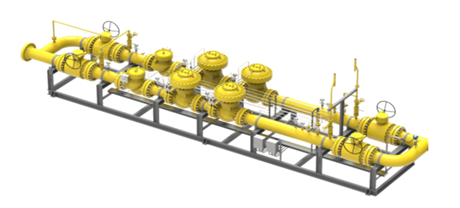
\includegraphics[width=0.7\textwidth]{assets/images/pressure_reduction_station.png}
	\caption{Pressure Reduction Station}
	\label{fig:your_image}
 \end{figure}


\section*{Application and Results}
{\fontsize{12}{12}\selectfont 
In order to indendfy the location of pump stations and pressure reduction stations, the elevations and the value which is gotten from Aspen HYSYS are used. The route of pipeline is shown in 2nd Picture:
\\

}

\begin{figure}[h!]
	\centering
	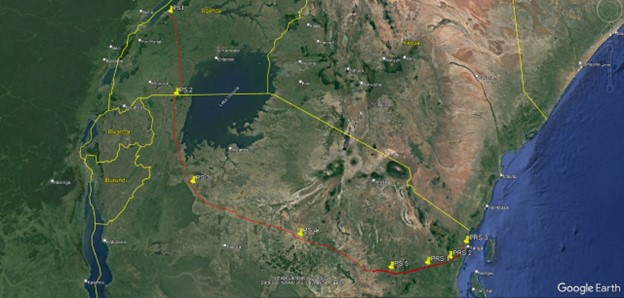
\includegraphics[width=0.7\textwidth]{assets/images/pipeline_route.jpg}
	\caption{Pipeline Route}
	\label{fig:your_image}
 \end{figure}


{\fontsize{12pt}{12pt}\selectfont 
While drawing simulation in Aspen HYSYS (3rd  Picture ) , firstly parameters for input have to be indicated. These parameters are components of oil, temperature, pressure, liquid flow of oil and it is illustrates in 4th Picture.
\\

}

\begin{figure}[h!]
	\centering
	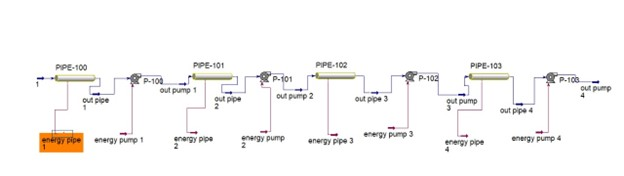
\includegraphics[width=0.7\textwidth]{assets/images/some_pipe_stuff.jpg}
	\caption{Aspen HYSYS Simulation }

	\vspace{10mm}

	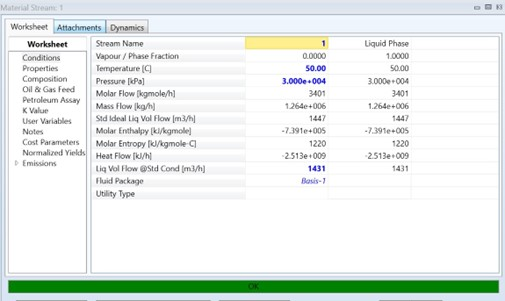
\includegraphics[width=0.7\textwidth]{assets/images/inlet.jpg}
	\caption{Conditions for inlet stream}
	\label{fig:your_image}
 \end{figure}
 

{\fontsize{12pt}{12pt}\selectfont
Consequently, remaining datas for example molar flow and mass flow is defined by Aspen HYSYS. And, for each pipeline the length, pressure drops whin that pipeline and related to that pressure loss the power of the pump is indicated table below which is calculated by Aspen HSYSY. 
\\


}


\section*{Discussion}
{\fontsize{12pt}{12pt}\selectfont
\hspace*{1em}In this section, the outcomes that are shown in the Results part are discussed and some problems related to project are addressed.Firstly, the one important sidegoal of the project is taking environmental risks such as contamination into consideration and minimizing the social impacts which are mainly disagreement between people.To achieve these,some essential steps are taken.As shown in Methodology section,to avoid those problems, the whole pipeline trajectory was remodeled.According to new design, trajectory does not cross any houses, schools and etc. so that there is no disturbtion to local communities.This step increases the route to 1500.2 km to our main route,however this alternative way saves approximately 90 million USD.Elevations across the route are considered.Although it adds extra cost to our budget, the money that is saved totally compensates it.Natural disasters, seasonal changes are mainly considered while choosing route.Route does not cross rivers to keep away from problems which are related to alterations when seasons change.The climate conditions which are extreme temperature changes, the disasters as floods, volcanic eruptions and others have to be prevented.
\\

Another important issue is about the pipeline itself.The material of the pipe should be chosen carefully and considering all the external impacts in long term.First thing that can weaken the pipeline is corrosion.The material should be resistant to harsh environments that can have soil , moisture ad etc.Material should be strong enough to  endure external forces such as pressure and temperature.Another point is compability.Material must have compatibility with the oil inside the pipe to avoid the chemical reactions that can make problems for the coherence of pipeline.As mentioned in Results part, Uganda oil has difficult properties.So the proper material that fits all the criterias above is chosen for this project.
\\

}

\section*{Conclusion}
{\fontsize{12pt}{12pt}\selectfont
\hspace*{1em} In conclusion,the highest point of this extensive report about the pipeline of oil project highlights the necessity of strategical arrangement,environmental awareness and cohesion to safety regulations in energy industry.Our main aim was to prepare the ideal pipeline route for carrying oil from Uganda to Tanzania by considering all the environmental and social impacts and the one that is cost-effective for our budget.The most proper route is created with the help of application called Google Earth Pro by our team members.Pipeline material is chosen carefully and knowing the values Diameter-0.6 m , Length -1500.2 km and others, pressure loss and head loss are calculated to be 65.658 Mpa and 7967.92 m respectively.

}




\end{document}
